\documentclass[11pt,a4paper]{article}
\usepackage[utf8]{inputenc}
\usepackage[vietnamese]{babel}
\usepackage{amsmath,amssymb}
\usepackage[version=4]{mhchem}
\usepackage{geometry}
\geometry{top=1.1cm,bottom=1.0cm,left=1.4cm,right=1.4cm,headheight=24pt,headsep=7pt,footskip=13pt}
\usepackage{graphicx}
\usepackage{xcolor}
\usepackage{tabularx}
\usepackage{array}
\usepackage{tikz}
\usepackage{multicol}
\usepackage{fancyhdr}
\usepackage{enumitem}

\definecolor{hfRed}{HTML}{D32F2F}
\definecolor{hfGreen}{HTML}{8BC390}
\definecolor{mainGreen}{HTML}{2E7D32}

\usepackage{ex_test}

\pagestyle{fancy}
\fancyhf{}
\renewcommand{\headrulewidth}{0.75pt}
\renewcommand{\headrule}{\hbox to\headwidth{\color{hfGreen}\leaders\hrule height \headrulewidth\hfill}}
\renewcommand{\footrulewidth}{0.75pt}
\renewcommand{\footrule}{\hbox to\headwidth{\color{hfGreen}\leaders\hrule height \footrulewidth\hfill}}

\fancyhead[L]{\small\itshape\color{hfRed}Tài liệu lưu hành nội bộ}
\fancyhead[R]{\small\color{hfRed}Thầy \textbf{TRẦN VĂN THẠNH} - 0777.470.803}

\fancyfoot[L]{\footnotesize\itshape\color{hfRed}CS1: 6/15 Nguyễn Hoàng, P. Kim Long, TP Huế \quad|\quad CS2: 24 Đặng Thái Thân, TP Huế}
\fancyfoot[R]{\small\textbf{\color{hfRed}Trang \thepage}}

\setlength{\parindent}{0pt}
\setlength{\parskip}{0.0pt}

\def\loigiai#1{}

\begin{document}

\Opensolutionfile{ans}[ans-de12-hs]

\noindent
\begin{minipage}[t]{0.48\textwidth}
	\textbf{SỞ GIÁO DỤC VÀ ĐÀO TẠO THỪA THIÊN HUẾ}\\
	\textbf{TRƯỜNG THPT HAI BÀ TRƯNG}\\
	\textbf{ĐỀ CHÍNH THỨC}\\
	\textit{(Đề thi có 04 trang)}
\end{minipage}\hfill
\begin{minipage}[t]{0.48\textwidth}
	\raggedleft
	\textbf{\color{mainGreen}ĐỀ KIỂM TRA ĐỊNH KỲ CHƯƠNG 4 (POLYMER)}\\
	\textbf{MÔN: HOÁ HỌC -- LỚP 12}\\
	\textit{Thời gian làm bài: 50 phút (không kể thời gian phát đề)}\\
	\textbf{Mã đề thi: 112}
\end{minipage}


\vspace{0pt}
\noindent\textit{Họ, tên thí sinh: \dots\dots\dots\dots\dots\dots\dots\dots\dots\dots\dots\dots\dots\dots\dots\dots\dots\dots\dots\dots\dots\dots Lớp: \dots\dots\dots\dots SBD: \dots\dots\dots\dots}\\
\noindent\textit{(Cho biết nguyên tử khối: H = 1; C = 12; N = 14; O = 16; Na = 23; Al = 27; S = 32; Cl = 35,5; K = 39; Ca = 40; Fe = 56; Cu = 64; Zn = 65; Br = 80; Ag = 108; Ba = 137).}

\vspace{1pt}
\noindent
\textbf{PHẦN I (4,5 điểm -- 18 câu): Câu trắc nghiệm nhiều phương án lựa chọn.}\\
\textit{Thí sinh trả lời từ câu 1 đến câu 18. Mỗi câu hỏi thí sinh chỉ chọn một phương án.}

\setcounter{ex}{0}

\begin{ex}
Tên gọi của polymer có công thức cho dưới đây là
\par{\centering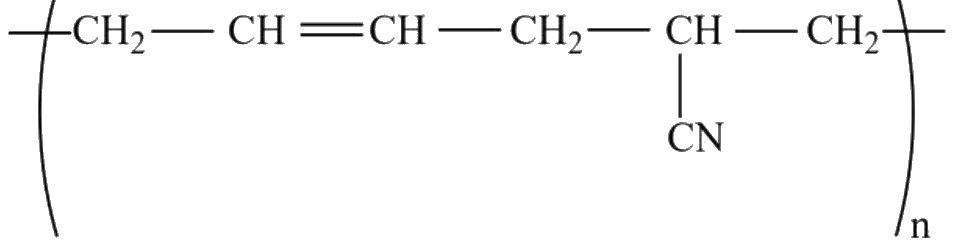
\includegraphics[height=0.8cm]{images_crop_de12/cau1_buna_n.png}\par}
\choice
{Cao su buna}
{Cao su buna-S}
{Cao su buna-N}
{Cao su isoprene}
\loigiai{}
\end{ex}

\begin{ex}
(SBT -- KNTT). Poly(vinyl chloride) (PVC) là một loại chất dẻo phổ biến, được sử dụng làm vỏ dây điện, ống dẫn nước thải, áo mưa, vải giả da,\dots{} PVC có công thức cấu tạo là
\choice
{$[-CH_2-CH_2-]_n$}
{$[-CH_2-CH(CH_3)-]_n$}
{$[-CH_2-CH(C_6H_5)-]_n$}
{$[-CH_2-CH(Cl)-]_n$}
\loigiai{}
\end{ex}

\begin{ex}
Polymer nào sau đây có thể cộng với hydrogen chloride?
\choice
{Polyacrylonitrile}
{Polyethylene}
{Polyisoprene}
{Tinh bột}
\loigiai{}
\end{ex}

\begin{ex}
Trong các phản ứng giữa các cặp chất dưới đây, phản ứng nào làm giảm mạch polymer?
\choice
{Poly(vinyl chloride) + \ce{Cl2}}
{Cao su thiên nhiên + \ce{HCl}}
{Tinh bột + \ce{H2O} ($t^\circ$, \ce{H+})}
{Poly(vinyl acetate) + \ce{NaOH}}
\loigiai{}
\end{ex}

\begin{ex}
(SBT -- KNTT). Polymer nào sau đây \textbf{không} thuộc loại chất dẻo?
\choice
{Poly(methyl methacrylate)}
{Poly(vinyl chloride)}
{Polystyrene}
{Polybuta-1,3-diene}
\loigiai{}
\end{ex}

\begin{ex}
(SBT -- KNTT). LDPE là một chất dẻo dễ tạo màng, có tính dai bền nên được sử dụng làm túi nylon, màng bọc, bao gói thực phẩm. Trên các bao bì làm từ LDPE thường được in kí hiệu như hình bên. LDPE được tổng hợp từ monomer nào sau đây?
\par{\centering
\includegraphics[height=0.85cm]{images_crop_de12/cau6_ldpe_symbol.png}\par}
\choice
{\ce{CH2=CH2}}
{\ce{CH2=CH-CH3}}
{\ce{CH2=CH-C6H5}}
{\ce{CH2=CHCl}}
\loigiai{}
\end{ex}

\begin{ex}
(SBT -- CTST). Nylon-6,6 thuộc loại tơ nào sau đây?
\choice
{Tơ polyester}
{Tơ bán tổng hợp}
{Tơ thiên nhiên}
{Tơ tổng hợp}
\loigiai{}
\end{ex}

\begin{ex}
(SBT -- CTST). Loại polymer thiên nhiên nào có thành phần chính là cellulose?
\choice
{Bông}
{Tơ tằm}
{Len}
{Cao su thiên nhiên}
\loigiai{}
\end{ex}

\begin{ex}
(SBT -- KNTT). Cao su buna-N (hay còn gọi là cao su nitrile, có kí hiệu là NBR) là loại cao su tổng hợp có khả năng chịu dầu mỡ tốt nên được dùng làm ống dẫn nhiên liệu, gioăng phớt làm kín trong các máy móc. Thực hiện phản ứng trùng hợp các chất nào dưới đây thu được sản phẩm là cao su buna-N?
\choice
{\ce{CH2=CH-CH=CH2} và \ce{C6H5CH=CH2}}
{\ce{CH2=C(CH3)-CH=CH2} và \ce{CH2=CHCN}}
{\ce{CH2=CH-CH=CH2} và \ce{N2}}
{\ce{CH2=CH-CH=CH2} và \ce{CH2=CHCN}}
\loigiai{}
\end{ex}

\begin{ex}
Nhận xét về tính chất vật lí chung của polymer nào dưới đây \textbf{không} đúng?
\choice
{Hầu hết là những chất rắn, không bay hơi}
{Đa số nóng chảy ở một khoảng nhiệt độ rộng, hoặc không nóng chảy mà bị phân hủy khi đun nóng}
{Đa số không tan trong các dung môi thông thường, một số tan trong dung môi thích hợp tạo dung dịch nhớt}
{Hầu hết polymer đều đồng thời có tính dẻo, tính đàn hồi và có thể kéo thành sợi dai, bền}
\loigiai{}
\end{ex}

\newpage

\begin{ex}
Dãy nào sau đây chỉ chứa các polymer thiên nhiên?
\choice
{Poly(vinyl chloride), tinh bột, cellulose}
{Protein, tinh bột, polyethylene}
{Protein, cellulose}
{Protein, tinh bột, cellulose}
\loigiai{}
\end{ex}

\begin{ex}
Cho dãy gồm các polymer: (1) polybuta-1,3-diene, (2) polyacrylonitrile, (3) poly(vinyl chloride), (4) poly(hexamethylene adipamide). Polymer bị thuỷ phân trong môi trường acid là
\choice
{(1)}
{(3)}
{(4)}
{(2)}
\loigiai{}
\end{ex}

\begin{ex}
Nhận xét nào sau đây đúng?
\choice
{Đa số các polymer dễ hòa tan trong các dung môi thông thường}
{Đa số các polymer không có nhiệt độ nóng chảy xác định}
{Các polymer đều bền vững dưới tác động của acid, base}
{Các polymer dễ bay hơi}
\loigiai{}
\end{ex}

\begin{ex}
Cho các polymer sau: polyethylene, poly(methyl methacrylate), poly(vinyl chloride), polyacrylonitrile. Số polymer điều chế được bằng phản ứng trùng hợp là
\choice
{3}
{4}
{1}
{2}
\loigiai{}
\end{ex}

\begin{ex}
Phát biểu nào sau đây sai?
\choice
{Tơ nitron thuộc loại tơ tổng hợp}
{Tơ nylon-6,6 thuộc loại tơ tổng hợp}
{Tơ visco thuộc loại tơ thiên nhiên}
{Tơ acetate thuộc loại tơ bán tổng hợp}
\loigiai{}
\end{ex}

\begin{ex}
Phát biểu sai là
\choice
{Bản chất cấu tạo hoá học của tơ tằm và len là protein; của sợi bông là cellulose}
{Bản chất cấu tạo hoá học của tơ nylon là polyamide}
{Quần áo nylon, len, tơ tằm không nên giặt với xà phòng có độ kiềm cao}
{Tơ nylon, tơ tằm, len rất bền vững với nhiệt}
\loigiai{}
\end{ex}

\begin{ex}
(SBT -- CTST). Trùng ngưng $\varepsilon$-aminocaproic acid thu được $m\text{ kg}$ capron và $12{,}6\text{ kg } \ce{H2O}$ với hiệu suất phản ứng 90\%. Giá trị của $m$ là
\choice
{71,19}
{79,10}
{91,70}
{90,40}
\loigiai{}
\end{ex}

\begin{ex}
Keo dán là vật liệu được sử dụng rộng rãi trong đời sống. Cho các phát biểu sau về keo dán:\\
(a) Keo dán là vật liệu có khả năng kết dính bề mặt của hai vật liệu rắn với nhau mà không làm biến đổi bản chất các vật liệu được kết dính.\\
(b) Nhựa vá săm là dung dịch dạng keo của chất dẻo trong dung môi hữu cơ như toluene, xylene, thường được dùng để vá chỗ thủng của săm xe.\\
(c) Keo dán epoxy còn gọi là keo dán một thành phần.\\
(d) Thành phần chính của keo epoxy là hợp chất chứa hai nhóm epoxy ở hai đầu. Thành phần thứ hai là chất đóng rắn, thường là các polyamine.\\
(e) Ưu điểm của keo epoxy là độ kết dính rất cao, chịu nhiệt, chịu nước, chịu dung môi, chịu lực tốt, rất dễ sử dụng. Keo epoxy thường được dùng để dán các kim loại, nhựa, bê tông, các vật bằng kính, sứ, gỗ, đồ gốm.\\
Số phát biểu đúng là
\choice
{2}
{3}
{5}
{4}
\loigiai{}
\end{ex}

\newpage

\noindent
\textbf{PHẦN II (4,0 điểm -- 4 câu): Câu trắc nghiệm đúng sai.}\\
\textit{Thí sinh trả lời từ câu 1 đến câu 4. Trong mỗi ý a), b), c), d) ở mỗi câu, thí sinh chọn đúng hoặc sai.}

\setcounter{ex}{0}

\begin{ex}
(SBT -- CTST). Tơ capron và polyacrylonitrile có công thức cấu tạo như hình dưới:
\par\vspace{1pt}{\centering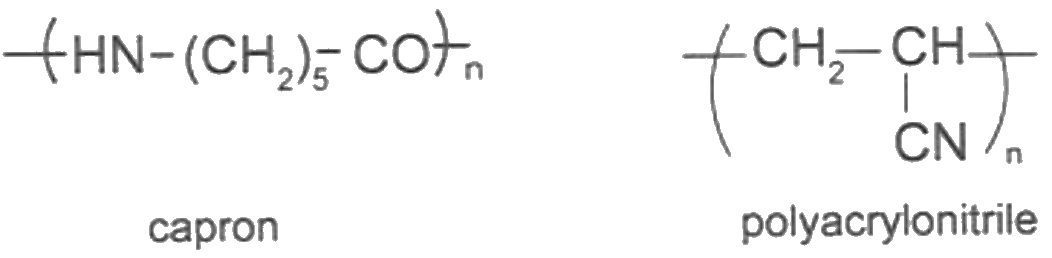
\includegraphics[height=1.0cm]{images_crop_de12/p2_cau1_polymers.png}\par}\vspace{1pt}
\choiceTF
{Cả hai loại đều dùng để chế tạo tơ}
{Polyacrylonitrile được điều chế bằng phản ứng trùng ngưng}
{Capron thuộc loại polypeptide}
{Hai polymer đều có phản ứng phân huỷ mạch trong môi trường kiềm}
\loigiai{}
\end{ex}

\begin{ex}
(SBT -- CĐ). Năm 1839, Charles Goodyear đã được cấp bằng sáng chế cho phát minh về quy trình hoá học để chế tạo ra cao su lưu hoá -- một loại cao su có cấu trúc đặc biệt, bền cơ học, chịu được sự ma sát, va chạm, đàn hồi tốt và có thể đúc được. Những phát biểu nào sau đây là đúng?
\choiceTF
{Cao su lưu hoá còn có tên gọi là cao su buna-S}
{Bản chất của việc lưu hoá cao su là tạo ra cầu nối disulfide \ce{-S-S-} giữa các mạch cao su nên cao su lưu hoá có tính chất cơ lí nổi trội hơn}
{Trong mủ cao su thiên nhiên, polymer có tính đàn hồi là polyisoprene}
{Cao su lưu hoá có cấu trúc mạng không gian nên bền hơn cao su chưa lưu hoá}
\loigiai{}
\end{ex}

\begin{ex}
Cây cao su là loại cây công nghiệp có giá trị kinh tế lớn, được đưa vào trồng ở nước ta từ cuối thế kỉ 19. Chất lỏng thu được từ cây cao su giống như nhựa cây (gọi là mủ cao su) là nguyên liệu để sản xuất cao su tự nhiên.
\choiceTF
{Thành phần chính của cao su thiên nhiên là polyisoprene có cấu hình dạng cis}
{Cao su thiên nhiên có tính đàn hồi, không có tính dẫn điện, không thấm khí và nước, không tan trong nước, nhưng tan nhiều trong xăng, benzene\dots}
{Cao su thiên nhiên có tính đàn hồi chỉ tồn tại trong khoảng nhiệt độ hẹp. Để cải thiện tính chất này người ta xử lý bằng cách trộn cao su thiên nhiên với styrene gọi là quá trình lưu hóa cao su}
{Mắt xích của cao su thiên nhiên được viết thu gọn là \ce{C5H8}}
\loigiai{}
\end{ex}

\begin{ex}
Bản chất kết dính của keo dán là tạo ra lớp màng mỏng bám chắc vào hai mảnh vật liệu để giúp chúng kết dính lại với nhau.
\choiceTF
{Keo dán poly(urea -- formaldehyde) được điều chế từ phản ứng trùng ngưng}
{Keo dán poly(urea -- formaldehyde) gồm phần chính là poly(urea -- formaldehyde) và thêm phần đóng rắn như oxalic acid, ammonium chloride\dots{} để tạo polymer có cấu trúc mạch phân nhánh}
{Keo dán epoxy có polymer mạng không gian với độ kết dính cao dùng để gắn kết hai bề mặt vật cần dán lại như kim loại, thủy tinh, gỗ\dots}
{Keo dán tổng hợp thông dụng thường gặp gồm keo dán urea -- formaldehyde, keo dán epoxy và nhựa vá săm}
\loigiai{}
\end{ex}

\newpage

\noindent
\textbf{PHẦN III (1,5 điểm -- 6 câu): Câu trắc nghiệm yêu cầu trả lời ngắn.}\\
\textit{Thí sinh trả lời từ câu 1 đến câu 6.}

\setcounter{ex}{0}

\begin{ex}
Cho dãy gồm các nguyên liệu: (1) $\varepsilon$-aminocaproic acid, (2) acrylonitrile, (3) $\omega$-aminoenanthic acid, (4) ethylene glycol và terephthalic acid, (5) hexamethylenediamine và adipic acid. Số nguyên liệu (hoặc cặp nguyên liệu) được dùng để tiến hành phản ứng trùng ngưng tạo thành tơ là
\par\noindent\textit{Trả lời:} \dotfill
\loigiai{}
\end{ex}

\begin{ex}
Cho các polymer: amylose (1); cao su isoprene (2); cellulose acetate (3); thủy tinh hữu cơ (4); tơ tằm (5). Số lượng polymer thiên nhiên là
\par\noindent\textit{Trả lời:} \dotfill
\loigiai{}
\end{ex}

\begin{ex}
Phân tử khối của một đoạn mạch tơ nylon-6,6 là 56 500 amu. Số lượng mắt xích trong đoạn mạch nylon-6,6 nêu trên là
\par\noindent\textit{Trả lời:} \dotfill
\loigiai{}
\end{ex}

\begin{ex}
Polystyrene (PS) là loại nhựa dùng chế tạo hộp xốp đựng thức ăn. Hãy tính hệ số polymer hóa của loại nhựa này khi biết phân tử khối của nó bằng 104 000 amu.
\par\noindent\textit{Trả lời:} \dotfill
\loigiai{}
\end{ex}

\begin{ex}
Trong công nghiệp, để điều chế cao su buna người ta có thể đi từ nguyên liệu khí ethylene thu được từ dầu mỏ theo sơ đồ:
$$2\,\ce{C2H4} \xrightarrow{(1)} 2\,\ce{C2H5OH} \xrightarrow{(2)} \ce{C4H6} \xrightarrow{(3)} \ce{[-CH2-CH=CH-CH2-]_n}\text{ (cao su buna)}$$
Tính thể tích khí ethylene (đo ở 25 $^\circ\text{C}$ và 1 bar) cần lấy để điều chế được 1 tấn cao su buna theo sơ đồ trên. Giả sử hiệu suất phản ứng của mỗi quá trình (1), (2) và (3) lần lượt là 65\%, 50\% và 70\% (kết quả làm tròn đến hàng đơn vị theo đơn vị $\text{m}^3$).
\par\noindent\textit{Trả lời:} \dotfill
\loigiai{}
\end{ex}

\begin{ex}
(SBT -- CĐ). Caprolactam được tổng hợp từ cuối thế kỉ XIX. Hiện nay, nhu cầu sản xuất caprolactam trên thế giới khoảng 10 triệu tấn/năm; 90\% trong đó dùng để tổng hợp tơ capron. Trong công nghiệp, caprolactam được điều chế theo sơ đồ sau:
\par\vspace{2pt}{\centering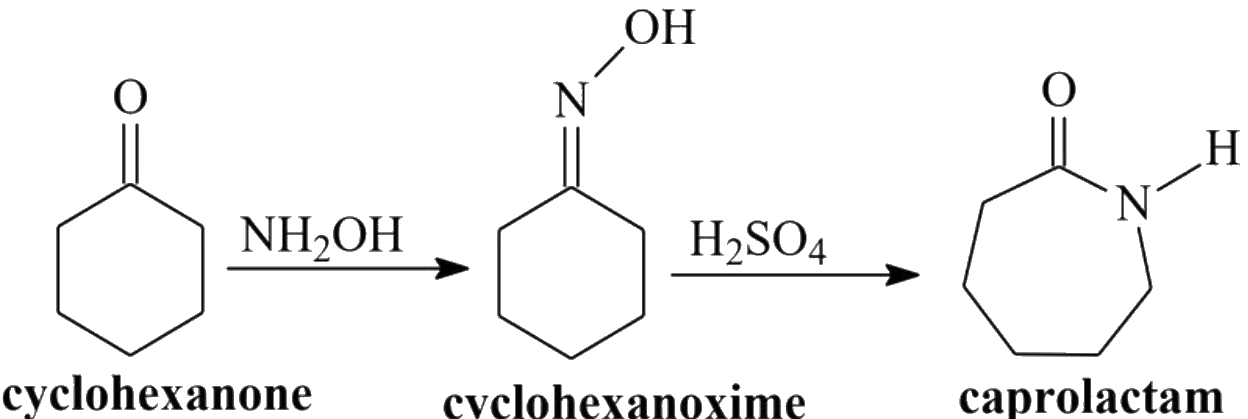
\includegraphics[height=1.8cm]{images_crop_de12/p3_cau6_caprolactam_scheme.png}\par}\vspace{2pt}
Để sản xuất 10 triệu tấn caprolactam, cần sử dụng bao nhiêu triệu tấn cyclohexanone (giả sử hiệu suất trung bình của cả quá trình trên là 60\%)? (Kết quả làm tròn đến chữ số hàng phần mười).
\par\noindent\textit{Trả lời:} \dotfill
\loigiai{}
\end{ex}


\Closesolutionfile{ans}

\end{document}
